%%
%% Author: melo
%% 16/08/2018
%%

%%%% PREAMBLE %%%%

%%% MASTER HEADER
%%
%% Author: Gabriel Melo
%% 05/08/2018
%%

% abntex2
\documentclass[11pt,openright,twoside,a4paper,brazil, article]{abntex2}

% Packages
\usepackage{a4wide}
\usepackage[margin=0in, ignorehead, left=3cm, right=2cm, bottom=3cm,top=2cm]{geometry}
\usepackage{lipsum}%% a garbage package you don't need except to create examples.
\usepackage{fancyhdr}
\usepackage{graphicx}
\usepackage{titlesec}
\graphicspath{ {./img/} }
\usepackage{layout} % Package that print the page dimensions (use \layout)
\usepackage{xcolor}
\usepackage{framed}
\definecolor{purple-emk}{RGB}{125,0,125}
\usepackage{multicol}
\setlength{\columnsep}{1cm}
\usepackage{enumerate} % To use roman characters on enumarated list

%% ROBOTO FONT (http://www.tug.dk/FontCatalogue/roboto/)
\usepackage[sfdefault]{roboto}  %% Option 'sfdefault' only if the base font of the document is to be sans serif
\usepackage[T1]{fontenc}


%% FIRST PAGE STYLE
\fancypagestyle{first_page}
{
\renewcommand{\headrulewidth}{0pt}
\fancyhf{}

\lhead{
\hspace{-207pt}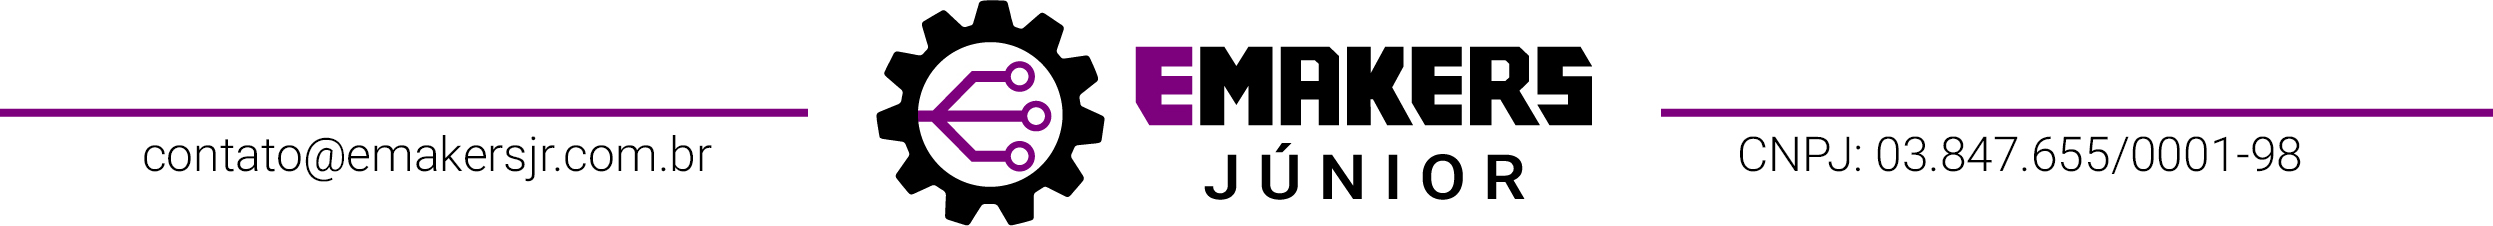
\includegraphics[scale=0.27]{header}
}

\lfoot{
\vspace{8pt}
\colorbox{purple-emk}{\textcolor{white!30}{\titulo \textcolor{purple-emk}{Ç}} \hspace{300pt}}
}

\rfoot{
\vspace{9pt}
\colorbox{black!90}{\textcolor{white!30}{ \hspace{15pt} Página \thepage} \hspace{15pt}}
}

\headheight 40pt
\headsep 0pt

}

%% ALL PAGES STYLE
\fancypagestyle{all_pages}
{
\renewcommand{\headrulewidth}{0pt}
\fancyhf{}

\lfoot{
\vspace{8pt}
\colorbox{purple-emk}{\textcolor{white!30}{\titulo \textcolor{purple-emk}{Ç}} \hspace{300pt}}
}

\rfoot{
\vspace{9pt}
\colorbox{black!90}{\textcolor{white!30}{ \hspace{15pt} Página \thepage} \hspace{15pt}}
}

\headheight 40pt
\headsep 0pt

}

%% ASSINGMENT COMMAND
\newcommand{\assigment}[2]{
\begin{center}
    \underline{\hspace{7cm}}

    #1

    #2

\end{center}
}


% New command to set text margin
%\def\changemargin#1#2{\list{}{\rightmargin#2\leftmargin#1}\item[]}
%\let\endchangemargin=\endlist

\setlength{\oddsidemargin}{15.5pt}
\setlength{\evensidemargin}{15.5pt}


%%% CONTRACT HEADER
%%
%% Author: Gabriel Melo
%% 05/08/2018
%%

%%% COUNTERS &&&
\newcounter{clausula_number}
\setcounter{clausula_number}{0}
\newcounter{paragrafo_number}
\setcounter{paragrafo_number}{0}

\makeatletter
\@addtoreset{paragrafo_number}{clausula_number}
\makeatother


%% CLÁUSULA COMMAND
\newcommand{\clausula}{
\stepcounter{clausula_number}
\section*{\hspace{-20pt} \textbf{CLÁUSULA  \arabic{clausula_number}º:}}\label{sec:Clausula\arabic{clausula_number}}
}

%% PARAGRAFO COMMAND
\newcommand{\paragrafo}{
\addtocounter{paragrafo_number}{1}
\section*{\hspace{-20pt} \textbf{§  \arabic{paragrafo_number}º:}}\label{sec:Paragrafo\arabic{paragrafo_number}-\arabic{clausula_number}}
}

%% SECAO COMMAND
\newcommand{\secao}[1]{
\begin{center}
    \textbf{#1}
\end{center}
}


%% ASSINGMENT SECTION COMMAND
\newcommand{\assigmentSection}{

\bigskip

\bigskip

\bigskip

\begin{multicols}{2}
    \begin{center}
        \textbf{CONTRATADA}

        \bigskip

        \bigskip

    \end{center}
    \signature{Gabriel Marques de Melo}{Diretor-presidente Emakers Júnior}

    \bigskip

    \bigskip

    \bigskip

    \begin{center}
        \textbf{TESTEMUNHA 1}

        \bigskip

    \end{center}

    Nome:

    \bigskip

    CPF:

    \bigskip

    RG:

    \bigskip
    \signature{}{}

    \begin{center}
        \textbf{CONTRATANTE}

        \bigskip

        \bigskip

    \end{center}
    \signature{\nome}{\profissao}

    \bigskip

    \bigskip

    \bigskip

    \begin{center}
        \textbf{TESTEMUNHA 2}

        \bigskip

    \end{center}

    Nome:

    \bigskip

    CPF:

    \bigskip

    RG:

    \bigskip

    \signature{}{}

\end{multicols}
}



%% CONTRATO'S COMMANDS
\newcommand{\contratada}{\section*{\hspace{-20pt} \textbf{CONTRATADA:}} Gabriel Marques de Melo, estudante, brasileiro, solteiro, residente e domiciliado à rua Comandante Vilas Boas, 29, Bairro Jardim Floresta, Lavras/MG, inscrito sob o CPF de nº 021.324.496-94 e RG de nº MG-16.191.021. }\label{Contratada}

\newcommand{\contratante}{
    \section*{\hspace{-20pt} \textbf{CONTRATANTE:}}\label{Contratante} \nome, \profissao, \nacionalidade, \estadoCivil, residente e domiciliado à \rua, \numero, \bairro, \cidadeUF, inscrito sob o CPF de nº \cpf e RG de nº \rg.

    \bigskip

    \noindent As partes acima identificadas firmam o presente contrato nos termos aqui ajustados.

}


% FORMAT CLAUSULA & PARAGRAFO TITLES
\titleformat{\section}[runin]
{\normalfont\bfseries}
{}{0pt}{}
\titlespacing{\section}
{\parindent}{*2}{\wordsep}

%% DADOS DO DOCUMENTO
\def\titulo{EDITAL GENÉRICO}

%% DADOS DO EDITAL
\def\projeto{Redação Inteligente}

\title{\titulo}
\author{Gabriel Marques de Melo}
%\date{}

%%%% END PREAMBLE %%%%

%%%% DOCUMENT %%%%
\begin{document}
	\initdoc

	A Emakers Júnior torna público o presente edital, com procedimentos para seleção do time de desenvolvimento responsáveis por implementar as funcionalidades do projeto \textbf{\textcolor{purple-emk}{\projeto}}, doravante aqui denominado PROJETO.

	\secao{DO OBJETO}
	\clausula O objetivo é selecionar, no máximo, 6 (seis) membros plenos da empresa para comporem o time de desenvolvimento do PROJETO.

	\secao{DO PROJETO}
	\clausula O projeto consiste em um aplicação web para submissão de redações por alunos e correção delas pelos professores, de forma automatizada.
	\clausula A Execução do projeto consiste em um serviço prestado pela Emakers Júnior a um cliente, sendo este um pessoa física.
	\clausula Os requisitos, com TODAS as funcionalidades que DEVEM ser cumpridas e implementadas, podem ser obtidos em:
	https://drive.google.com/open?id=17XS9HoQKm0eh-EeHM1oln-ugxqB4N4sb0wzw9NJvhsc

	\secao{DOS PRAZOS}
	\clausula O prazo final de entrega do produto COMPLETO, é dia 7 de janeiro de 2019, conforme previsto em contrato.

	\paragrafo No decorrer do desenvolvimento, segundo a metodologia Scrum, haverão sub-prazos a serem cumpridos, as Sprints.

	\paragrafo Todo o desenvolvimento do projeto obedecerá ao disposto na metodologia ágil da empresa, disponível em:

	%https://drive.google.com/open?id=1xU4qtqDhZoxXpDjI2KVOWJ5mV_SZrCkEk15t4ITPL60
	
	%https://drive.google.com/open?id=1rM7gVzj6Pag0UyfFBu-rAEFyqx4Duj4TRYV1wXP8DOo

	\secao{DO CARGO}

	\clausula A vigência do cargo começa assim que for divulgado o resultado e termina no dia 7 de janeiro de 2019, prazo final de entrega do projeto.

	\clausula Em caso extraordinário, a data de vigência poderá ser alterada caso a mudança seja devidamente aprovada pela Diretoria Executiva da Emakers Júnior.

	
	\secao{DO TIME DE DESENVOLVIMENTO}

	\clausula O time de desenvolvimento será composto por todos os desenvolvedores selecionados neste edital.

	\clausula O time, como um todo, deverá prezar pelo cumprimento dos itens 2.3 e 2.4 com excelência e profissionalidade.

	
	\secao{DA INSCRIÇÃO}

	\clausula Qualquer membro efetivo da Emakers Júnior, excetuando o gerente do projeto,  podem candidatar-se à vaga.
	
	\clausula A inscrição é feita pelo preenchimento do formulário: 
	https://goo.gl/forms/JLEmOwDO78R4sjQj2

	\clausula O prazo inicia-se com a publicação deste, até as 18:00 do dia 16 de agosto de 2018, quinta-feira.


	\secao{DO RESULTADO}
	\clausula O resultado será divulgado no dia 17 de agosto de 2018, sexta-feira, a partir das 11:00.


	\secao{DAS DISPOSIÇÕES GERAIS}
	
	\clausula O Gerente do projeto, juntamente com o Diretor de Projetos, avaliará e selecionará o(s) candidato(s) que melhor se encaixe(m) no perfil do cargo para o projeto, seguindo o que foi disposto no regimento interno da empresa.
	
	\clausula Não cabe recurso sobre o resultado final, pois a decisão é do Gerente do projeto.
	
	\clausula Qualquer dúvida deve ser encaminhada ao canal \textbf{\#dúvidas} do Slack da Emakers Júnior.



\end{document}